\chapter{Methoden und Techniken} \label{cha:Methoden}
    In diesem Kapitel soll es um die verwendeten Methoden und die grundlegenden Bedingungen zur Untersuchung von Molekülen auf antiferromagnnetischen Oberflächen gehen.
    Hierfür sind oberflächensensitiv Methoden wie die Photoelektronenspektroskopie von großer Bedeutung.
    Notwendig dafür ist ein Ultrahochvakuumsystem mit Drücken unterhalb von \SI{1e-9}{\milli\bar}~\cite{Henzler}.
    Diese tiefen Drücke sind erforderlich, da schon bei einem Druck von \SI{1e-6}{\milli\bar} die Oberfläche innerhalb von \SI{10}{\milli\second} zu \SI{1}{\percent} mit den im Restgas vorhandenen Teilchen bedeckt wäre~\cite{Henzler}.
    Grundlegend ist es mit ihr möglich sich den für die elektrische Leitfähigkeit relevanten Bereich genauer anzuschauen. 
    Aber auch die Aussagen über die chemischen Zusammensetzungen des untersuchten Systems sind damit möglich.
    Diese grundlegenden Prinzipien werden im \autoref{sec:PES} behandelt.
    Zusätzlicher Informationsgewinn über die Verteilung und die Dispersions der Ladungen in der Probe können durch die Erfassung des Austrittswinkels erlangt werden (siehe \autoref{sec:PEEM}).
    Die Erforschung von selbstanordnen Molekülen auf Oberflächen nehmen einen immer größeren Bereich in der Wissenschaft ein. 
    Zur Identifizierung der beteiligten Molekülorbital eignet sich die Photoemissionsorbitaltomographie die in \autoref{sec:MOT} eingeführt wird.

    \section{Photoelektronenspektroskopie} \label{sec:PES}
        % Die Grundlage der Photoelektronenspektroskopie ist der photoelektrische Effekt, der 1905 zum ersten Mal von Albert Einstein erklärt wurde~\cite{Einstein}.
        Die Photoelektronenspektroskopie gibt Aufschluss über die elektronische Struktur innerhalb eines Festkörpers.
        Hierzu werden monochromatische Photonen einegstrahlt, die durch den photoelektrischen Effekt Elektronen anregen.
        Für eine ausreichend hohe Energie der Photonen ist es möglich die Elektronen aus dem Festkörper zu lösen und zu detektieren.
        Dazu muss das Photon der Energie $h \nu$ die Bindungsenergie des Elektrons $E_\text{B}$ sowie die Austrittsarbeit der Probe $\phi$ überwinden.
        Die restliche zur Verfügung stehende Energie wird als kinetische Energie
        \begin{equation}
            E_{\text{Kin}} = h \nu - E_{\symup{B}} - \phi
            \label{eqn:Photoeffekt}
        \end{equation}
        an das Elektron abgegeben.
        Da die Austrittsarbeit die Energiedifferenz zwischen Ferminiveau der Probe und Vakuumniveau darstellt bezieht sich die kinetische Energie immer auf die Vakuumenergie.
        Im Gegensatz dazu bezieht sich die Bindungsenergie auf die Fermienergie ($E_\text{B} = \num{0}$ bei $E_\text{F}$) und wird für gebundene Zustände stets positiv dargestellt.

        \begin{figure}
            \centering
            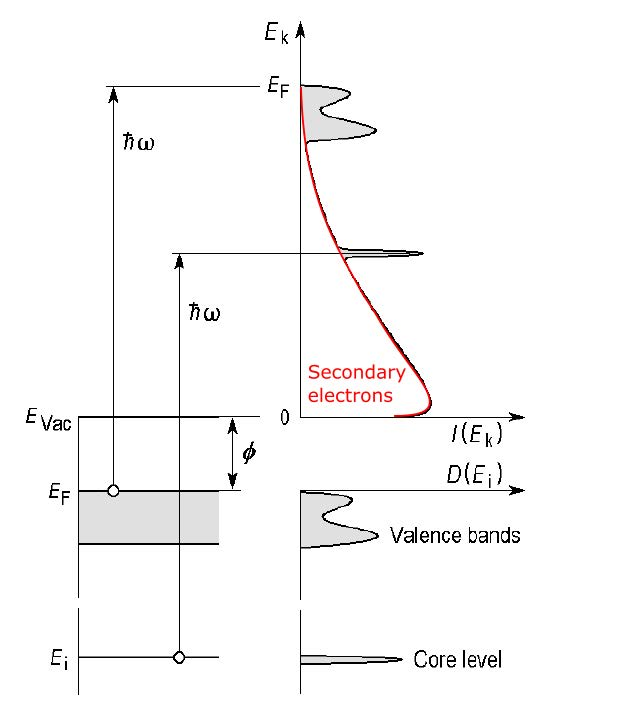
\includegraphics[width=0.5\textwidth]{EDC_DJ.jpg}
            \caption{Kopiert aus \cite{oura_surface_2003}.}
            \label{fig:EDC}
        \end{figure}
        Wird die Anzahl detektierter Elektronen gegen ihre kinetische Energie aufgetragen, so ergibt sich die Energie Verteilungsfunktion (\textit{energy distribution curve}, EDC).
        Diese spiegelt die Zustandsdichte der entsprechenden Probe wieder, beispielhaft ist dies in \autoref{fig:EDC} dargestellt.
        Links im Bild ist die elektronische Struktur in einem Festkörper dargestellt, rechts die sich ergebene Energie Verteilungskurve.
        Mit Hilfe der Röntgenstrahlung (\textit{X-Ray}) können sich kernnahe Zustände untersucht lassen, welche Rückschlüsse auf die chemische Zusammensetzung der Probe zulassen (\textit{Electron spectroscopy for chemical analysis}, ESCA).
        Ihre Struktur ist im Vergleich zu der des Valenzbandbereiches schmaler.
        Der Valenzbandbereich nahe der Fermikante lässt sich mittels der ultravioletten Strahlung genauer untersuchen.
        Ihre Strukturen fallen dabei eher etwas breiter aus als die der Kernniveaus.
        Die verschiedenen Energiebereiche sind notwendig, damit die angeregten Elektronen eine kinetische Energie im oberflächensensitiven Bereich haben.
        Diese erste Methode wird XPS (siehe \autoref{sec:XPS}) genannt, wohingegen die zweite Methode mit UPS (siehe \autoref{sec:UPS}) abgekürzt wird.
        Durch die zusätzliche Erfassung der Austrittswinkel der Elektronen kann die Bandstruktur wieder gegeben werden, dazu wird die winkelaufgelösten UPS genutzt (siehe \autoref{sec:ARPES}).
        
        \begin{figure}
            \centering
            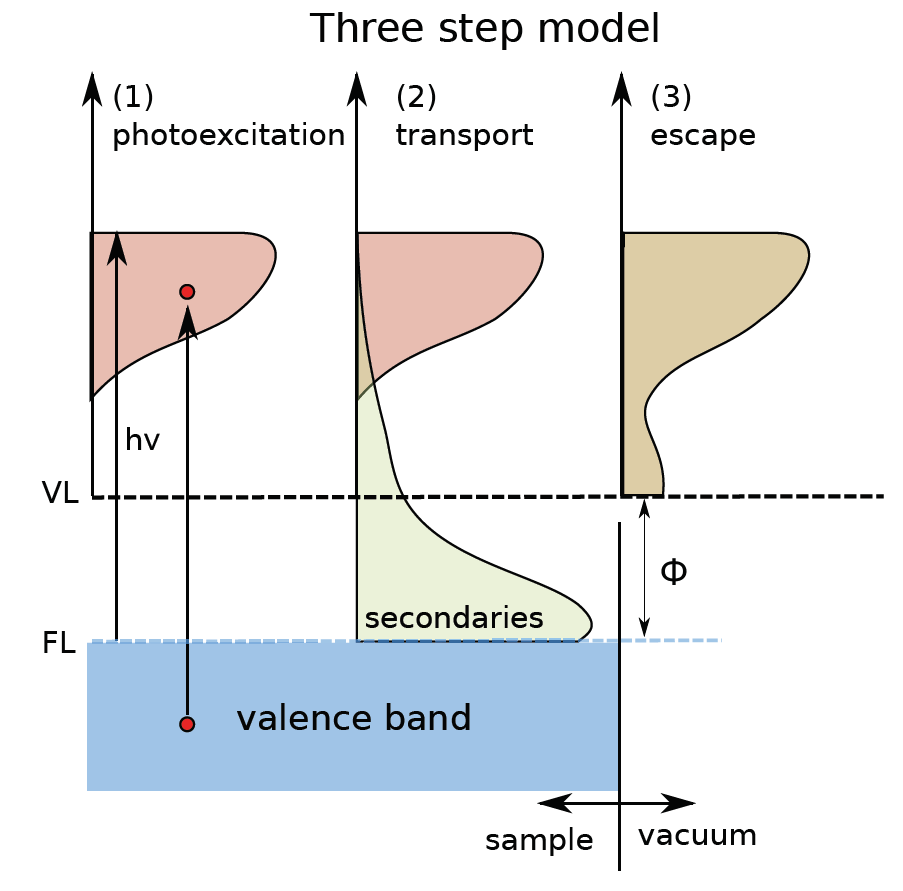
\includegraphics[width=0.5\textwidth]{3Stufen}
            \caption{Schematische Darstellung des drei Stufen Models für den photoelektrischen Effekt.
            Bestehend aus (1) Absorption, (2) Transport zur Oberfläche und (3) Austritt aus der Oberfläche.
            Kopiert und modifiziert aus~\cite{zhang_synchrotron_2018}.}
            \label{fig:3Stufen}
        \end{figure}
        \begin{figure}
            \centering
            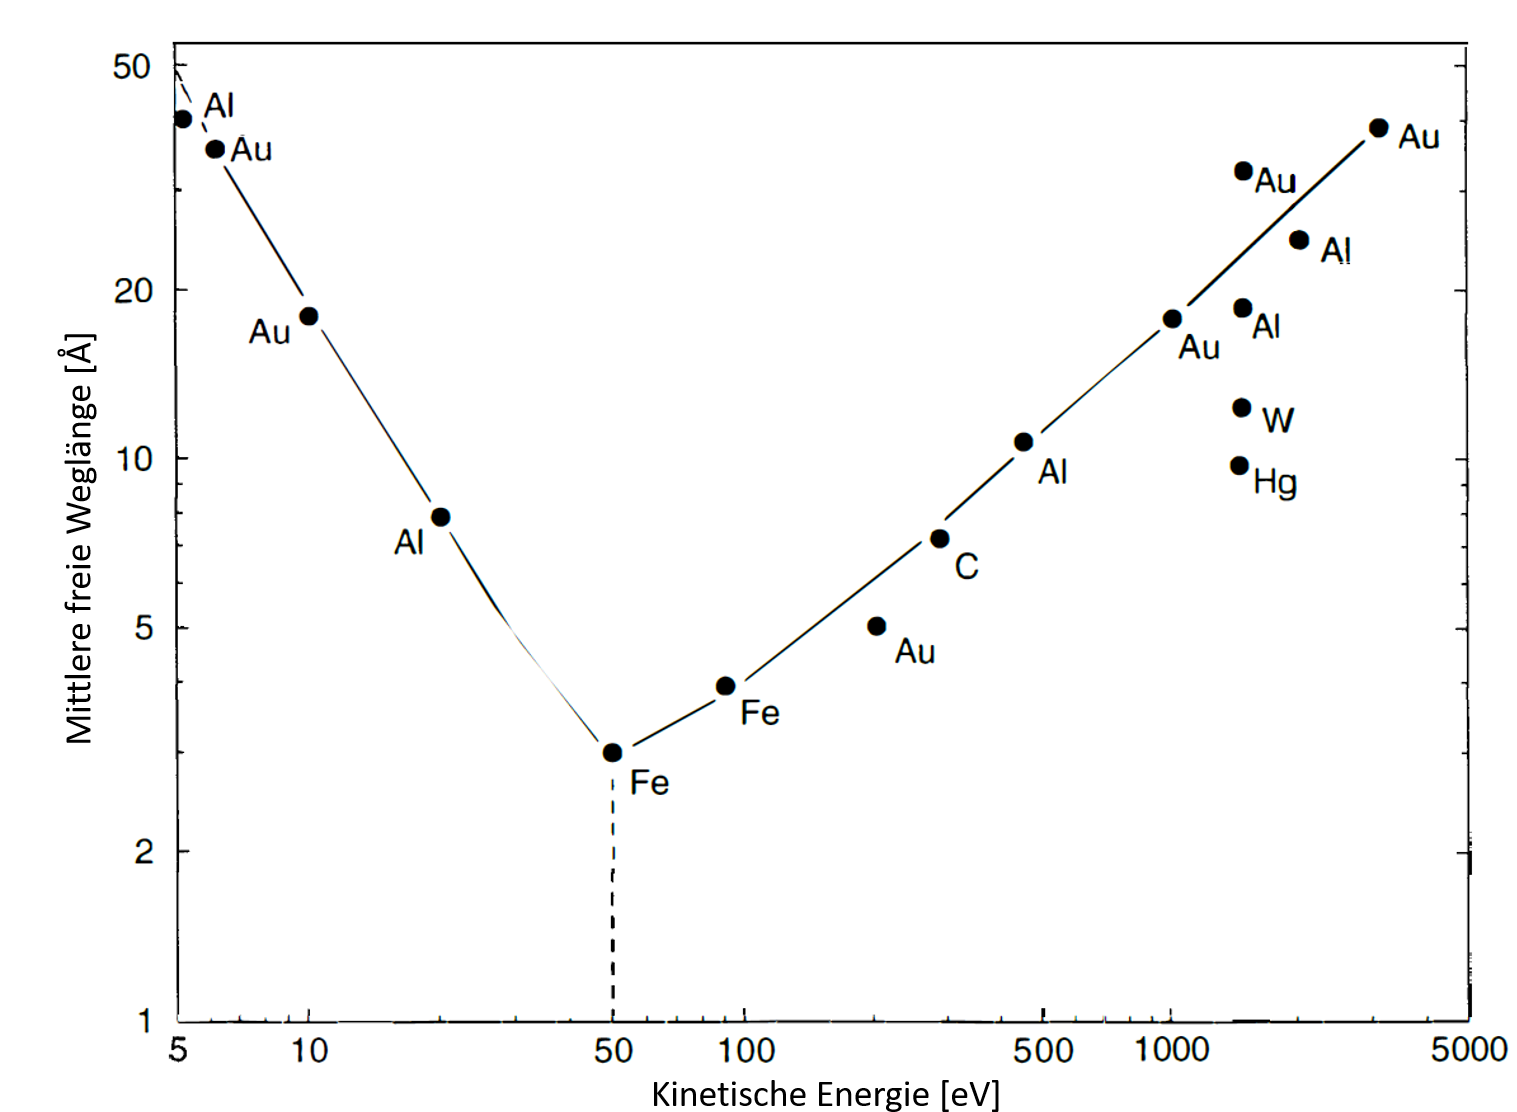
\includegraphics[width=0.6\textwidth]{Weg2.png}
            \caption{Die mittlere freie Weglänge für Elektronen in verschiedenen Materialien. Aus~\cite{Hüfner} und bearbeitet.}
            \label{fig:Weg}
        \end{figure}
        Dieser Prozess der Photonelektronenemission lässt sich in einem Model mit drei unabhängigen Stufen erklären.
        Das Model ist in \autoref{fig:3Stufen} schematisch zu sehen.
        Der erste Schritt ist die Absorption des Photons, wodurch das Elektron aus seiner Bindung gelöst werden kann und mit einer kinetischen Energie versehen wird.
        Dieses kann dann innerhalb des Festkörpers zur Probenoberfläche wandern.
        Auf dem Weg zur Oberfläche können die  Elektronen hauptsächlich mit anderen Elektronen stoßen, wodurch es im Fall eines elastischen Stoßes Energie und damit seine Informationen seines Ursprungs verliert.
        Die gestreuten Elektronen erzeugen einen kontinuierlichen Untergrund und ihr Beitrag steigt mit abnehmender kinetischen Energie an, sie werden auch Sekundärelektronen genannt.
        Ein Maß für die Strecke die ein Elektron ohne Energieverlust durchlaufen kann, wird inelastische mittlere freie Weglänge genannt.
        Diese ist von der kinetischen Energie des Elektrons abhängig und in \autoref{fig:Weg} dargestellt.
        Es ist zu erkennen, dass Elektronen mit einer kinetischen Energie im Bereich von \SIrange{30}{100}{\electronvolt} aus einer Tiefe von nicht mehr als \SI{5}{\angstrom} kommen und somit aus dem Oberflächen nahen Bereich.
        Ist die kinetische Energie des Elektrons größer als die Austrittsarbeit der Probe, so kann das Elektron die Oberfläche in einem dritten Schritt verlassen.
        An der Oberfläche des Festkörpers ist die Periodizität gebrochen, wodurch das Elektron gebeugt wird und die senkrechte Komponente des Impulsvektors nicht erhalten bleibt.
        Dahingegen bleibt der Impulsvektor parallel zur Oberfläche $k_{||}$ erhalten, dies wird bei der winkelaufgelösten Photoelektronenspektroskopie in \autoref{sec:ARPES} zu Nutzen gemacht.

        Die Wahrscheinlichkeit für einen Übergang aus dem Anfangszustand $\Psi_\text{i}$ (i = \textit{intinal}) in einen weiteren Endzustand $\Psi_\text{f}$ (f = \textit{final}) wird durch Fermi's goldene Regel festgelegt.
        Damit ist auch die Intensität des Photoemissionsprozesses 
        \begin{equation}
            I_\text{fi} \propto \frac{2\pi}{\hbar} \abs{\bigl<\Psi_\text{f}|\Delta|\Psi_\text{i}\bigr>}^2 \, \delta\left(E_\text{f}-E_\text{i}-h\nu\right)
            \label{eqn:Fermi_gold}
        \end{equation}
        abhängig von der verwendeten Photonenenergie $h \nu$ und dessen klassische Vektorpotential des externen elektrischen Feldes $\vec{A}$, sowie der Energie des Anfangszustandes $E_\text{i}$ und Endzustandes $E_\text{f}$.
        Hierbei stellt $\Delta \approx \frac{\symup{e}\hbar}{m}\vec{A}\cdot\vec{p}$ einen Operator da und beschreibt die Interaktion zwischen dem äußeren Feld und dem Elektron~\cite{cao_theory_2010}.
        Der Übergang wird also durch die Symmetrien des Anfangs- und Endzustands bestimmt, ferner ist auch die Polarisation des einfallenden Photons entscheident.
        Die $\delta$-Funktion berücksichtigt das Prinzip der Energierhaltung.
        Um Elektronen mittels der Photoelektronenspektroskopie zu detektieren muss der Endzustand dabei oberhalb der Vakuumenergie liegen.
        Bei den durch das Photon angeregten Übergängen handelt es sich um direkte Übergänge und damit Impuls ($\vec{k}$) erhaltenen Prozess.
        Der Wellenvektor des Endzustandes $\vec{k}_\text{f}$ unterscheidet sich nur um einen reziproken Gittervektor $\vec{G}$ vom Wellenvektor des Anfangszustands $\vec{k}_\text{i}$.

        % Lokale Effekte vernachlässigt, N Elektronen im Anfangszustand

        Ein weiteres aktuelleres Model zur Beschreibung der theoretischen Photoelektronenemeission ist das ein Stufen Model.
        Diese fasst alle drei Elemente des drei Stufen Models zu einem zusammen, vobei der Endzstand durch einen Zustand beschrieben wird, der sich im Vakuum frei ausbilden kann aber in Richtung der Oberfläche gedämpft wird.
        Das ein Stufen Model behandelt den Prozess der Photoemission als einen kohärenten Prozess des Mehrteilchen Problems.
        Zusätzlich berücksichtigt es auch, dass sich der Grund- und Endzustand durch die Anregung und Erzeugung eines Lochs unterscheiden.

        \subsection{Röntgenphotoelektronenspektroskopie - XPS} \label{sec:XPS}
            Um die Kernniveaus des untersuchten Systems zu betrachten wird weichen Röntgenstrahlung mit einer Energie von \SIrange{0.1}{10}{\kilo\electronvolt} verwendet~\cite{Fauster}.
            Diese Energien sind nur mit klassischen Röntgenquellen oder einem Synchrotron erreichbar.
            Mit dieser Methode lässt sich die chemische Zusammensetzung der Probe untersuchen, da die typischen Bindungsenergien größer als \SI{50}{\electronvolt} sind und amit nicht direkt an Bindungen beteiligt sind.
            % und damit direkten Zugang zu der chemischen Komposition der Probe liefern.
            Leicht unterschiedliche Positionen in der Bindungsenergie für verschiedene Ionisationszustände und Bindungszuständen können dabei Rückschlüsse auf die chemische Umgebungen zulassen.
            Hierbei entsteht ein Beitrag auch durch die unterschiedlichen Bindungsenergien für die Atome an der Oberfläche oder tiefer im Festkörper liegend.
            Auf Grund der Symmetrien der Wellenfunktion der Kernniveaus ist ihre Bindungsenergie unabhängig vom Impulsvektor und das Signal zeigt die Form einer Lorentz-Funktion~\cite{Hüfner}.

            Maßgeblich wird die Halbwertsbreite des Signals durch die Lebenszeit des entsprechenden Zustands bestimmt, dabei ergibt sich eine inverse Proportionalität.
            Auch die Energieauflösung des Dektors fließt mit in die gemessene Halbwertsbreite ein, welches die bestimmte kinetische Energie beeinflusst.
            Die Halbwertsbreite der verwendeten Photonenenergie sorgt für unterschiedliche kinetische Energien der vom gleichen Zustand emittierten Elektronen.
            Durch vermessen des Systems bei niedrigen Temperaturen kann eine Verbreiterung des Siganls auf Grund von der Reduktion thermischer Effekte reduziert werden.
            Vermehrt treten bei Metallen einseitige Verbreiterungen auf, welche auf die Wechselwirkung zwischen dem Valenzband und dem im Kernniveau erzeugten Loch zurückzuführen ist.
            Durch dieses zusätzliche positive Potential führt zu einer Verschiebung zu größeren Bindungsenergien.
            % inelastische Streuungen der Photoelektronen zurückzuführen ist.
            Ebenso kann eine mehrfach Ionisation durch Multiphotonenabsorption oder interne Prozesse wie den Augerprozess zu Energieverschiebungen der emittierenden Zustände und damit einer Asymmetrie führen.
            % \textbf{???} Die Linien erfahren eine weiter Verbreiterungen, wenn sich durch die Spin-Bahn-Kopplung Dubletts ausbilden und nur eine geringe Energieaufspaltung zeigen.
            % Diese Aufspaltung resultiert aus der Wechselwirkung zwischen dem Spin des Valenzbandes und des photoionisierten Kernniveaus, was nun auch einen Spin trägt.

        
        % \subsection{Röntgenabsorptionspektroskopie - XAS}
        %     Für die Durchfürung von Röntgenabsorptionsmessungen ist eine durchstimmbare Photonenquelle im weichen Röntgenbereich notwendig.
        %     Dies ist aktuell nur durch Synchrotrons und Freieelektronenlaser realisierbar.
        %     Hierbei wird die Photonenenergie $h\nu$ über einen bestimmten Bereich variiert. % in der eine Abosrptionskante liegt abgetastet.
        %     Trifft ein Photon auf die Oberfläche so wird dieses absorbiert und kann ein Photoelektron auslösen.
        %     Wie viele Photonen diesen Prozess anregen können hängt davon ab, ob sich Elektronen bei der Energie $h\nu = E_\text{B}+\phi$ befinden.
        %     Energien an den schlagartig die Absorption steigt werden auch Absorptionskanten genannt und sind charakteristisch für verschiedene Elemente. 
        %     Es handelt sich dabei dann um einen Übergang aus einem bestimmten kernnahen Zustand in einen unbestzten Zustand.
        %     Durch die Wahl der Polarisation des Lichtes kann auch spinsensetiv selktiert werden, welche Elektronen ausgelöst werden.

        \subsection{Ultraviolettphotoelektronenspektroskopie - UPS} \label{sec:UPS}
            Das Valenz- und Leitungsband kann mit ultravioletter Strahlung im Bereich von \SIrange{10}{100}{\electronvolt} untersucht werden~\cite{Fauster}.
            Photonen in diesem Energiebereich können in Laboren mit Gasentladungslampen erzeugt werden, sind aber ebenfalls an Synchrotrons verfügbar.
            Durch die niedrige Photonenenergie ist die Wechselwirkungswahrscheinlichtkeit mit den entsprechenden Zuständen größer, als bei der Verwendung von Röntgenstrahlung.
            In diesen Bereich fallen auch die Energien die zur Photoemissionsorbitaltomographie genutzt werden, welche in \autoref{sec:MOT} eingeführt wird.

            Aufgrund der starken $\vec{k}$-Abhängigkeit im Valenzband und dessen Erhaltung, sowie der niedrigen Photonenenergien können bei der Ultraviolettphotoelektronenspektroskopie einige Zustände nicht abgebildet werden~\cite{Hüfner}.
            Bei XPS hingegen ist kaum eingeschränkt, denn durch die hohen Energien kann die ganze Brillouinzone als Akzeptanzbereich genutzt werden~\cite{Hüfner}.

        \subsection{Winkelaufgelöste Photoelektronenspektroskopie - ARPES} \label{sec:ARPES}
            Durch die Erfassung der Austrittswinkel der emittierten Elektronen lassen sich Rückschlüsse auf die Bandstruktur innerhalb der Probe schließen.
            Hierzu wird vom Analysator nur ein kleiner Winkelbreich akzeptiert und der Winkel zwischen Probe und Analysator stets variiert.
            Schematisch ist dies in \autoref{fig:ARPES} dargestellt.
            Für jede Winkelkombination aus polarem $\theta$ und azimunthalen $\phi$ Winkel wird ein UPS Spektrum aufgezeichnet.
            Die entsprechenden Impulsvektoren lassen sich aus den Winkeln und der kinetischen Energie nach
            \begin{gather}
                k_\text{x} = \sqrt{\frac{2 \text{m}_\text{e} E_\text{Kin}}{\hbar^2}} \sin\theta \cos\phi \\
                k_\text{y} = \sqrt{\frac{2 \text{m}_\text{e} E_\text{Kin}}{\hbar^2}} \sin\theta \sin\phi
            \end{gather}
            berechnen~\cite{MM_4}.
            Bei Messungen wird ein kleiner Teilbereich von $k_\text{||} = \sqrt{k_\text{x}^2 + k_\text{y}^2}$ erfasst.
            Mit verschiedene kinetische Energien aufgenommen ergibt sich damit ein Teilbereich der Bandstruktur $E(k_\text{||})$.
            Zusätzlich kann aus der Breite des Spektrums $\increment E$, also dem Beginn der Fermikante bis zum Abbruch der Sekundärelektronen die Austrittsarbeit der Oberfläche $\phi = h \nu - \increment E$ bestimmt werden~\cite{Hüfner}.
            % Durch die Korrelation zwischen dem Impuls und der kinetischen Energie
            % \begin{equation}
            %     E_\text{Kin} = \frac{\hbar^2 \vec{k}^2}{2 m_\text{e}}
            % \end{equation}
            % über das reduzierte planksche Wirkungsquantum $\hbar$ und der Elektronenmasse $m_\text{e}$
            % 
            % Im ein Stufen Model ergibt sich
            Unter Berücksichtigung der Austrittswinkel der Elektronen (polar $\theta$ und azimuthal $\phi$) sowie den finale Zustand $\Psi_\text{f}$ mit einer Energie $E_\text{Kin}$, die Photoelektronenintensität in entsprechende Richtung
            \begin{equation}
                I(\theta, \phi, E_\text{Kin}) \propto \sum_i \abs*{\bigl<\Psi_\text{f}(\theta, \phi, E_\text{Kin})|\vec{A}\cdot\vec{p}|\Psi_\text{i}\bigr>}^2 \times \delta\left(E_\text{i}+E_\text{Kin}+\Phi-h\nu\right))
            \end{equation}
            vom Anfangszustand $\Psi_\text{i}$ in der Dipolapproximation~\cite{MM_2}.

    \section{Photoelektronenemissionsmikroskopie} \label{sec:PEEM}
        Die Photoelektronenemissionsmikroskopie ist eine sehr viel versprechende Technik, die für immer mehr Aufsehen in den letzten Jahren gesorgt hat.
        Der größte Vorteil liegt wohl in der Kombination von spektroskopischen Methoden und mikroskopischen Methoden.
        Zuerst wurde dies 1933 durch E. Brüche entdeckt, der eine Zinkplatte mit Hilfe von Photoelektronen und einer magnetischen Linse auf einem Leuchtschirm abbildete~\cite{bruche_elektronenmikroskopische_1933}.
        Sie nutzt die Prinzipien der Energie- und Impulserhaltung um Bilder der Proben im Realraum oder Impulsraum aufzulösen.

        \begin{figure}
            \centering
            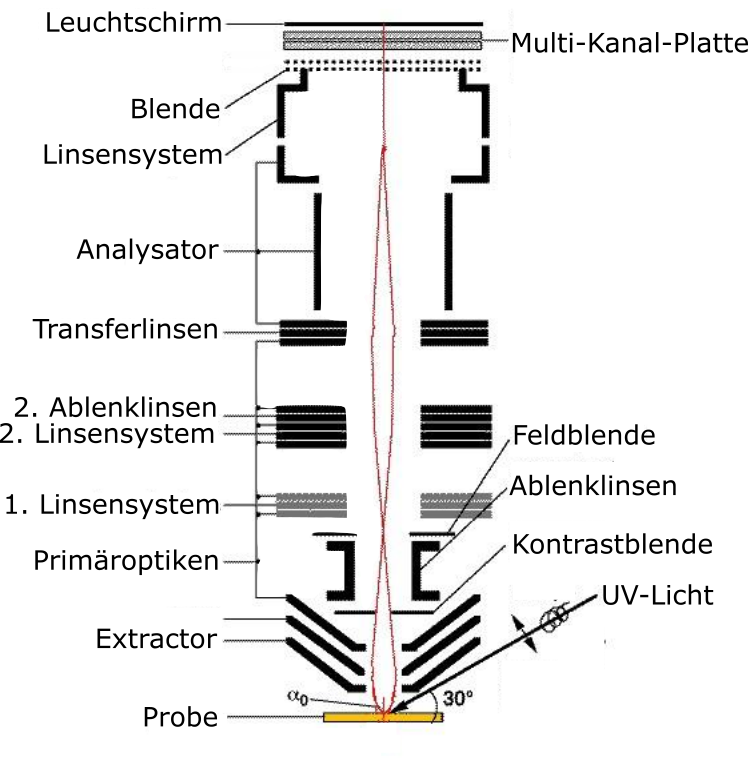
\includegraphics[width=0.6\textwidth]{PEEM_schemaneu.png}
            \caption{Vereinfachter Aufbau eines 2D Photoelektronen Mikroskopes. Vorlage aus~\cite{KUCH}, modifiziert.}
            \label{fig:MM}
        \end{figure}
        Ein exemplarischer Aufbau ist in \autoref{fig:MM} zu sehen.
        Die durch die Photonen angeregten Elektronen werden durch ein starkes elektrisches Feld von einigen \si{\kilo\volt} von der Probe zum Analysator hin beschleunigt.
        Das Extraktorfeld kann bis auf \SI{29}{\kilo\volt} erhöht werden.
        Durch diese große Spannung zwischen Probe und Extraktor ist es möglich einen großen Sichtbereich im Impulsraum abzudecken.
        Dies ist nötig, da durch den streifenden Einfall der Photonen und der Abberation der elektrostatischen Linsen nur einen kleinen Akzeptanzwinkel zur Verfügung stehen würde.
        Wichtig bei der Kathodenlinse ist, dass das Feld zwischen Probe und Linse sehr homogen ist, damit der Austrittswinkel erhalten bleibt, dies hat zur Folge, dass die Probe auch eine möglichst ebene Oberfläche aufweisen muss.
        Anschließend werden die Elektronen durch elektrostatische Linsen fokussiert und durch einzelne optische Elemente geleitet.
        Zusätzlich gibt es im Linsensystem noch elektrostatische Verschiebungslinsen, welche den Strahl ablenken und zentrieren.
        Die ersten Linsen sind so konzipiert, dass die Bildebene und die hintere Brennebene immer an der selben Position auftreten.
        An diesen beiden Stellen kann eine Blende eingestzt werden, die entscheidet ob sich ein Bild im Realraum oder im Impulsraum auf den Detektor abbildet.

        Im Anschluss an das erste Linsensystem folgt ein weiters Linsensystem aus elektrostatischen Linsen, welche das Bild auf den Ausgang des Linsensystems fokussieren.
        Hier befinden sich zwei magnetische Verschiebungslinsen um Drift zu korrigieren.
        Im Anschluss gehen die Elektronen in ein Transferlinsensystem über, welches dafür sorgt, dass ein einszueins Abbild auf die Eingangsblende des Analysators trifft.
        Die Eingangsblende kann in ihrer Größe variiert werden, sodass nur ein Teil der Elektronen in den Analysator eintritt.
        Je kleiner die Blende gewählt wird, desto besser ist die Energieauflösung aber so kleiner die Gesamtintensität.
        Als Energieanalysator kommt ein hemisphärischer Analysator zum Einsatz.
        Bei dem hemisphärischer Analysator werden die Elektronen zwischen zwei Halbkugeln durch ein statisches elektrisch Feld auf eine Kreisbahn gezwungen.
        Dabei ist das Feld so gewählt, dass nur die mit der richtigen kinetischen Energie eintretenden Elektronen auf die Austrittsblende abgebildet werden.
        % Ferner wird der Analysators so eingestellt, dass Elektronen mit einer Energie von \SI{50}{\milli\electronvolt} um die eingestellte Energie den Analysator passieren können, dies ist die Pass-Energie.
        
        Nach dem Detektor gibt es eine weiter Linseneinheit, welche zusammen mit einer Blende das gewünschte energieaufgelöst Bild auswählt und es auf die Detektorgröße aufweitet.
        Anschließend durchlaufen die Elektronen eine Mikrokanalplatte (eine Art Elektronenvervielfacher) und prallen auf den Phosphorschirm, der an den entsprechenden Stellen aufleuchtet.
        Durch die Kamera wird dieses Leuchten regestriert und das räumliche oder rekrusive Bild kann rekostruiert werden~\cite{SPECS-MM}.
        % Bei dem Detektor handelt es sich um eine CMOS Kamera die das Bild der auf den Leuchtschirm auftreffenden Elektronen aufnimmt.
        CCD (\textit{Charge Coupled Device}) Detektoren sind ein Standard bei ARPES Messungen, sie integrieren die analoge Photonenintensitäten oder einzelne Lichtblitze werden aufgezeichnet.
        Einer der Nachteile ist die geringe Abtastrate auf Grund der hohen Erholungszeit.
        Hier wird allerdings eine CMOS (\textit{Complemantary metal-oxid-semiconductor}) Kamera verwendet.
        % Dabei wird ein einzelnes Bild in nur wenigen Millisekunden erfasst, dies ist durch die Kombination von Kamera und Grafigprozessor möglich.
        Der Vorteil der CMOS Kamera Technik gegenüber der klassischen CCD  Kamera Technik ist, die Erfassung der wahren Pulszählraten~\cite{CMOS}.
        
        Es gibt zwei verschiedene Betribsmodi welche ferner erläutert werden.
        \begin{figure}
            \centering
            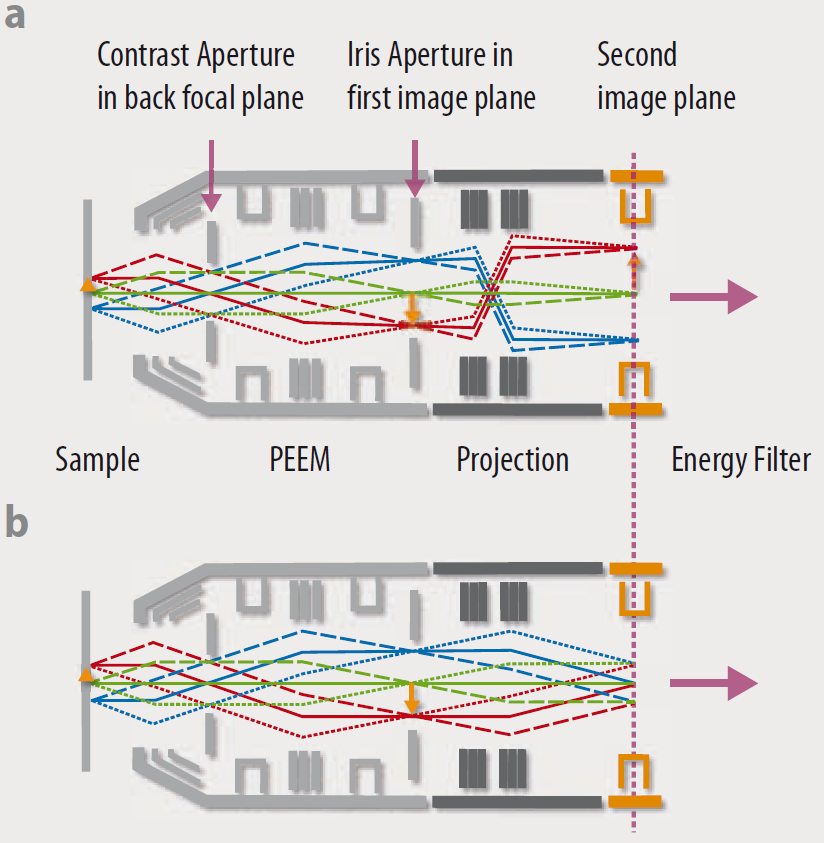
\includegraphics[width=0.5\textwidth]{Real_k.PNG}
            \caption{Die verschiedenen Konfiguration der Blenden um zwischen Realraum und Impulsraum Bild umzuschalten. Aus~\cite{Focus}.}
            \label{fig:real_k}
        \end{figure}
        Für den Impulsraum ist dies in \autoref{fig:real_k}\,a und für den Realraum in \autoref{fig:real_k}\,b dargestellt.
        Vorteil der Umschaltung zwischen den Modis ist, dass auf sehr kleinen Bereichen die im Realraum bestimmt wurden dann auch Messungen im reziproken Raum durchgeführt werden können.


        \subsection{Impulsraum Aufnahmen}
            Um ein Bild im Impulsraum aufzunehmen wird die Blende in der Bildebene eingefahren, die so genannte Feldblende (\textit{field aperture}).
            Durch die Blende wird ein Ausschnitt auf der Probe ausgwählt, von der die emittierten Elektronen erfasst werden.
            Bei einem Blendendurchmesser von \SI{20}{\micro\meter} und der Vergrößerung (\textit{magnification}) von~\num{5} ist der ausgewählt Bereich etwa \SI{4}{\micro\meter} groß.
            Bei der Aufnahme im Impulsraum wird bei der gesamten Abbildungsoptik der Austrittswinkel erhalten.
            So wird auf die Eintrittsblende des Analysators das Beugungsbild abgebildet.
            Das verwendete Mikroskop kann einen Austrittswinkel von biszu $\pm\SI{90}{\degree}$ erfassen für eine Energie kleiner als \SI{50}{\electronvolt}~\cite{SPECS-MM}.
            Für größere kinetische Energien wird das Sichtfeld auf $\pm\SI[per-mode=reciprocal]{3.6}{\per\angstrom}$ beschränkt.
            Dabei spielt es keine Rolle wo auf der Probe die Elektronen emittiert werden.

            Dies wird auch Impuls Mikroskopie (\textit{Momentum Microscopy}) bezeichnet.
            Bei der Impuls Mikroskopie ist die zeitgleich Erfassung des polaren und azimuntalen Austrittswinkel von großer Bedeutung. 
            So entsteht durch die zusätzlich Sortierung der Elektronen nach ihrer kinetischen Energie ein dreidimensionaler Datensatz.
            Wird über das gesamte Bild also alle Winkel integriert so ergibt sich die Kurve der Elektronendichte.

        \subsection{Realraum Aufnahmen}
            Es ist ferner möglich Bilder im Realraum aufzunehmen.
            Dies geschieht durch Einsetzen einer Blende in dem hinteren Brennpunkt, die Kontrastblende (\textit{contrast aperture}).
            Dabei können sehr kleine Spots von \SIrange{50}{200}{\micro\meter} ausgewählt werden.
            Um den Kontrast im Bild zu erhöhen werden nur Elektronen mit einem bestimmten Austrittswinkel für die Erstellung des Bildes erfasst.
            Mit Hilfe der Kontrastblenden kann eine Auflößung von einigen \si{\nano\meter} erreicht werden. 
            Auf dem Eintrittsspalt des Energieanalysators wird das Bild der Oberfläche projeziert.
            Das Bild wird bei festen Energiefilter-Einstellungen aufgenommen.
            Der Modi wird auch als PEEM (\textit{Photon emitted electron microscopy}) bezeichnet.
        
    \section{Photoemissionsorbitaltomographie} \label{sec:MOT}

    Durch die ebene Wellen Approximation des Endzustands ist der Photoelektronenstrom proportinal zur Fouriertransformation des Anfangszustandes.
    So ergibt sich unter Beachtung des Polarisationsfaktors $\abs*{\tilde{\Psi}_\text{i}(\vec{k})} \propto \frac{\sqrt{I_\text{i}(\theta, \phi)}}{\abs*{\vec{A}\cdot\vec{k}}}$.



        Die Photoemissionsorbitaltomographie vereinigt die Vorteile der Impulsmikroskopie mit der Dichtefunktionaltheorie (DFT) um Molekülorbitale zu identifizieren.
        Aus der Theorie können die Orbitale der Moleküle in der Gasphase im Realraum berechnet werden~\cite{database}.
        Werden diese dann Fourier transformiert, so ergibt sich die Aufenthaltswahrscheinlichkeiten der Elektronen abhängig von ihrem Impuls.
        Nun können die Moleküle bei einer bestimmten kinetischen Energie geschnitten werden und es ergibt sich ein zweidimensionales Bild~\cite{brandstetter_kmappy_2021}.
        Ferner kann auch die Wechselwirkungswahrscheinlichtkeit mit der verwendeten Photonenenergie berücksichtigt werden.
        Aus Messungen im Impulsraum können dann durch einen Vergleich die Molekülorbitale zugeordnet werden.
        Dies ist nur möglich, wenn sich die Moleküle ordnen wie z.B. auf einigen metallischen Oberflächen.

        Wie bereits in \autoref{sec:ARPES} erwähnt ist der Photoelektronenstrom in der Approximation einer ebenen Welle des Endzustands durch die Fouriertransformation des Anfangszustands verknüpft.
        So kann also durch erneute Fouriertransformation aus dem Impulsraum zurück in den Realraum auf die Molekülorbitale geschlossen werden~\cite{MM_2}.

        Unter der Beachtung von: (i)~der Emission von $\pi$-Orbitalen großer Moleküle, (ii)~dass der Winkel zwischen Polarisationsvektor $\vec{A}$ und Richtung der austretenden Elektronen $\vec{k}$ klein ist und (iii)~die Moleküle aus leichten Atomen bestehen, ist es möglich mit der Annahme der ebenen Welle und DFT die Molekülstruktur im Realraum zu berchnen \cite{MM_2}.
        \begin{figure}
            \centering
            \begin{subfigure}{0.3\textwidth}
                \centering
                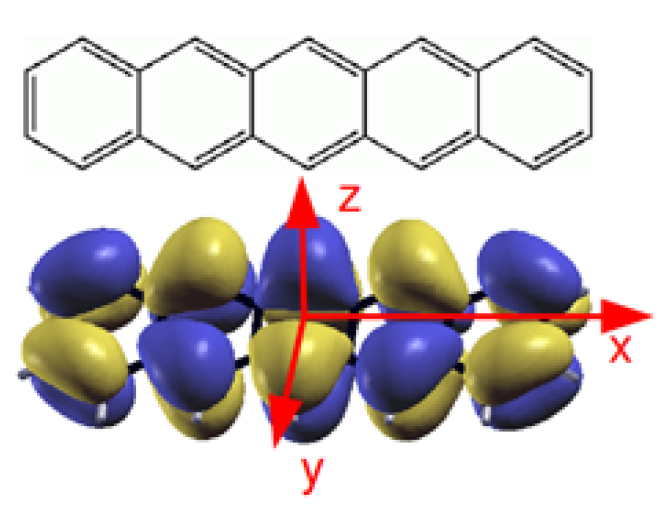
\includegraphics[width=0.9\textwidth]{DFT1.PNG}
                \caption{}
                \label{fig:DFT1}
            \end{subfigure}
            \begin{subfigure}{0.3\textwidth}
                \centering
                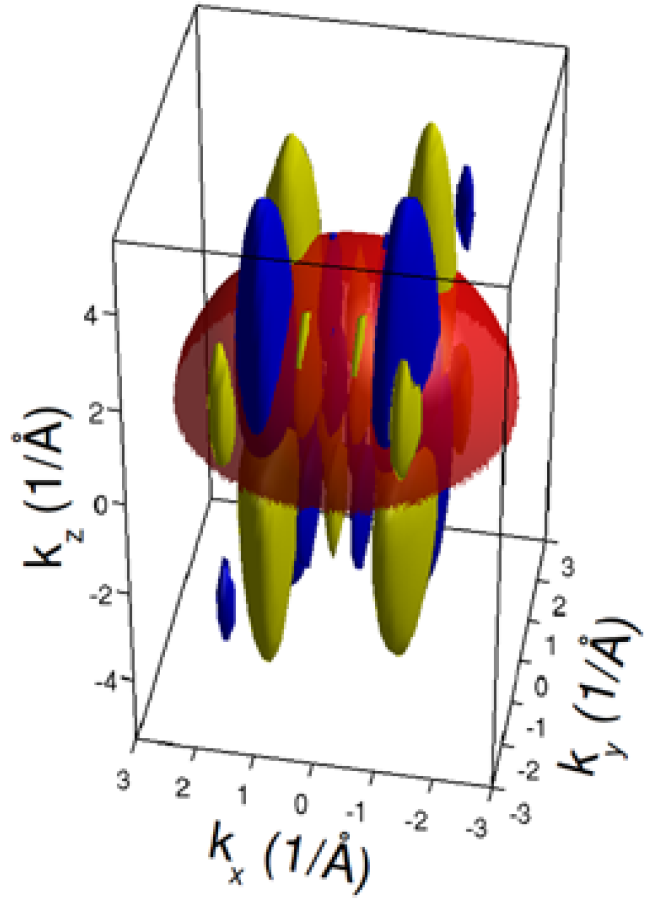
\includegraphics[width=0.9\textwidth]{DFT2.PNG}
                \caption{}
                \label{fig:DFT2}
            \end{subfigure}
            \begin{subfigure}{0.3\textwidth}
                \centering
                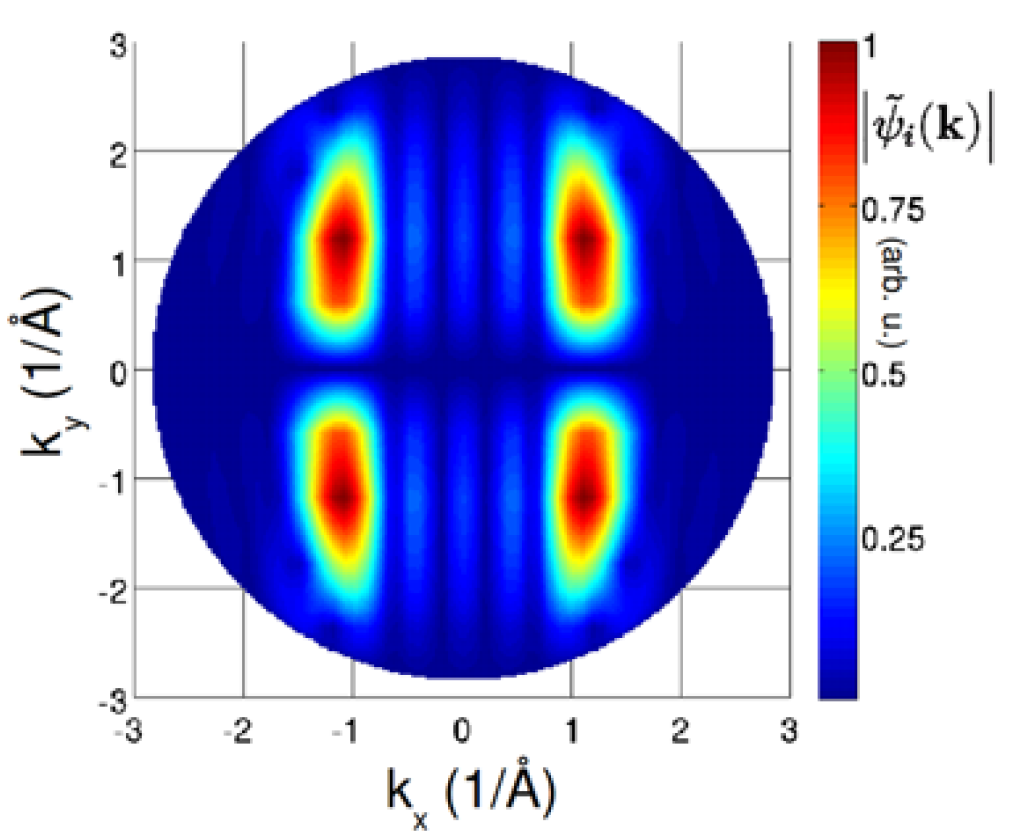
\includegraphics[width=0.9\textwidth]{DFT3.PNG}
                \caption{}
                \label{fig:DFT3}
            \end{subfigure}
            \caption{In (\subref{fig:DFT1}) ist die sich aus der Dichtefunktionaltheorie (DFT) ergebene Struktur von Pentacene gezeigt.
            Die durch Fouriertransformation gewonnen Orbitalstruktur im reziproken Raum (\subref{fig:DFT2}).
            (\subref{fig:DFT3}) die Projektion der Fouriertransformation der Molekülorbitale für eine feste kinetische Energie.
            Aus~\cite{MM_2}}
            \label{fig:DFT}
        \end{figure}
        Dies ist beispielhaft in \autoref{fig:DFT1} für Pentacene geschehen.
        Wird nun eine Fouriertransformation durchgeführt ergibt sich das Bild \autoref{fig:DFT2}.
        Schließlich wird die Fouriertransformation entlang einer Ebene konstanter kinetischer Energie, was der roten Hemisphäre in \autoref{fig:DFT2} entspricht, geschnitten.
        Es ergibt sich die Projektion in \autoref{fig:DFT3}.
        Nun kann diese Projektion mit der gemessenen Photoelektronenintensitäten verglichen werden.

        Mit Hilfe der Photoemissionsorbitaltomographie ist es nicht nur möglich Merkmale im Valenzband einzelnen Molekülorbitalen zuzuordnen, sondern auch ihre Ausrichtung auf dem Substraht zu bestimmen.
        So kann zum Beispiel die Neigung der Moleküle in eine Verschiebung der projezierten Molekülorbitalmerkmale in den Impulsbildern enden.
        Auch kann die Ausrichtung der Moleküle entlang der Symmetrien des Substrahtes bestimmt werden.

    \section{Versuchsaufbau}
    \label{sec:Versuchsaufbau}
        \begin{figure}
            \centering
            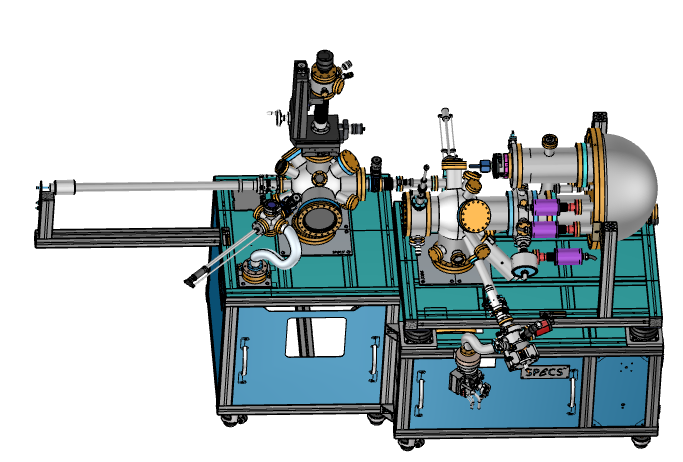
\includegraphics[width=0.7\textwidth]{MM.png}
            \caption{Der für die durchgeführten Experimente verwendete Aufbau.}
            \label{fig:aufbau}
        \end{figure}
        Um die in dieser Arbeit untersuchten Proben zu präperieren und zu untersuchen wird der Versuchsaufbau in \autoref{fig:aufbau} verwendet.
        Dieser besteht aus einer Präperationskammer (links im Bild) und dem 2D Photoelektronen Mikroskop KREIOS 150MM von SPECS (rechts im Bild).

        Für die Reinigung der Probe steht eine Ionenquelle zur Verfügung, um die Probe mittels ioneninduzierter Zerstäubung zu reinigen.
        Auf dem Manipulator, mit dem die Probe im Ultrahochvakuum verfahren werden kann, ist eine Elektronenstoßheizung montiert, um die Probe aufzuheizen.
        Die Präperationskammer ist mit einer LEED-Optik ausgestattet um die Oberflächenbeschaffenheit zu kontrollieren.
        Ferner befindet sich noch ein Leckventil für Sauerstoff, sowie Molekül- und Metallaufdampfer an der Kammer.
        
        Vor der Extraktorlinse des 2D Photoelektronen Mikroskopes befindet sich eine 6-Achsen-Piezostage (Hexapod) mit der die Probe in Position gebracht und ausgerichtet werden kann.
        Messungen erfordern eine exakte Ausrichtung der Oberflächennormalen parallel zur Linsenachse und ferner einen Abstand von \SI{4}{\milli\meter} zum Extraktor.
        Mit dieser Positioniereinheit kann die Probe auch auf unter \SI{10}{\kelvin} abgekühlt werden.
        Als Photonenquelle steht eine Helium-Gasentladungslampe bereit, welche größtenteils Photonen der He-I-Linie (\SI{21.22}{\electronvolt}) emittiert~\cite{UVS}.